\documentclass{ctexart}
\usepackage[a4paper,total={6in,8in}]{geometry}
\usepackage{fancyhdr}
\usepackage[table,xcdraw]{xcolor}
\usepackage{diagbox}
\usepackage[utf8]{inputenc}
\usepackage{ctex}
\usepackage{color}
\usepackage{subfigure}
\usepackage{cite}
\usepackage{graphicx}
\usepackage{fontspec}
\setmainfont{Times New Roman}
\newfontfamily\timesfont{Times New Roman}
\usepackage{CJK}
\usepackage{indentfirst}
\usepackage{amsmath}
\usepackage{mathrsfs}
\usepackage{multirow}
\usepackage{svg}
\usepackage{amsfonts}
\usepackage{geometry}
\usepackage{hyperref}
\usepackage{mathabx}
\usepackage{cases}
\definecolor{cherry}{HTML}{c93756}
\usepackage{minipage-marginpar}
\usepackage{xcolor}
% 导入包
\usepackage{hyperref}
% 格式设置
\hypersetup{hidelinks,
	colorlinks=true,
	allcolors=blue,
	pdfstartview=Fit,
	breaklinks=true}



\begin{document}

\begin{titlepage}
    \title{{\fontsize{28}{32}\selectfont\kaishu 机器人学 \\ \fontsize{20}{24}\selectfont\kaishu{作业5:运动学轨迹规划}}}
    \date{} % delete date as you want
    \maketitle
    \vspace{-7em}
    \begin{center}
      \fontsize{18}{22}\selectfont
      \textbf{\timesfont Robotics (2023-2024-2) \\
      Homework 5: Kinematic Trajectory Planning}
    \end{center}
    
    \begin{figure}[h]
        \centering
        
\includegraphics[width=0.45\textwidth]{Image/校标-校徽.png}
    \end{figure}
    \begin{center}
      \hspace{6em}
      \renewcommand{\arraystretch}{2}
      \begin{tabular}{rl}
      \fontsize{16}{50}\selectfont\heiti 姓名:& \fontsize{16}{24}\selectfont\heiti 赵四维 \\
      \fontsize{16}{24}\selectfont\heiti 学号:& \fontsize{16}{24}\selectfont 521021910696 \\
      \fontsize{16}{24}\selectfont\heiti 班级:& \fontsize{16}{24}\selectfont ME3403-01 \\
      \fontsize{16}{24}\selectfont\timesfont E-mail:& \fontsize{16}{24}\selectfont racheus.11@sjtu.edu.cn \\
      \end{tabular}
    \end{center}
    \begin{center}
      \fontsize{16}{24}\selectfont\timesfont \today
    \end{center}
\end{titlepage}

\pagenumbering{arabic}

\newpage
% \tableofcontents


\newpage
\pagestyle{fancy}
\fancyhf{}
\fancyhead[L]{ME3403-01}
\fancyhead[C]{机器人学Homework5}
\fancyhead[R]{赵四维 521021910696}
\fancyfoot[C]{\thepage}
\section{三次样条轨迹计算}
对于一个单自由度的连杆,对运动角度轨迹规划为两段三次样条曲线,运动开始与结束时速度为0,且在中间点速度与加速度连续,已知初始角度为$\theta_0$,中间角度为$\theta_1$,终止角度为$\theta_2$。
\begin{equation*}
	\begin{aligned}
		&Trajectory1: & \theta(t) = a_{10} + a_{11}t + a_{12}t^2 + a_{13}t^3 \\
		&Trajectory2: & \theta(t) = a_{20} + a_{21}t + a_{22}t^2 + a_{23}t^3	
	\end{aligned}
\end{equation*}
每段曲线的计算时间区间为:$t=0 \sim t_{fi}$,其中$i=1,2$,计算$t=t_{f1}=t_{f2}$时八个参数的计算表达式。

\subsection*{[Solution]:}
笔者最先做的时候没有考虑$t=t_{f1}=t_{f2}$的情形,因此求解了通解,过程如下:

由第一段样条曲线可知:
\begin{equation}
	\left\{
		\begin{aligned}
			\theta(0) &= a_{10} = \theta_0 \\
			\theta(t_{f1}) &= a_{10} + a_{11}t_{f1} + a_{12}t_{f1}^2 + a_{13}t_{f1}^3 = \theta_1 \\
			\dot{\theta}(0) &= a_{11} = 0 \\
			\dot{\theta}(t_{f1}) &= a_{11} + 2a_{12}t_{f1} + 3a_{13}t_{f1}^2
		\end{aligned}
	\right.
\end{equation}

上述方程组(1)解决了两个未知数$a_{10}$和$a_{11}$,接下来求解第二段样条曲线:
\begin{equation}
	\left\{
		\begin{aligned}
			\theta(0)&=a_{20}=\theta_1 \\
			\theta(t_{f2})&=a_{20}+a_{21}t_{f2}+a_{22}t_{f2}^2+a_{23}t_{f2}^3=\theta_2 \\
			\dot{\theta}(0)&=a_{21}\\
			\dot{\theta}(t_{f2})&=a_{21}+2a_{22}t_{f2}+3a_{23}t_{f2}^2=0\\
		\end{aligned}
	\right.
\end{equation}

上述方程组(2)解决了两个未知数$a_{20}$,接下来,还有5个未知数,我们需要建立\textcolor{red}{5个线性无关的方程},才能完全求解。

由方程组(1),将$a_{10}$和$a_{11}$代入,得以得到
\begin{equation}
	a_{12}t_{f1}^2+a_{13}t_{f1}^3=\theta_1-\theta_0
\end{equation}

由于转折位置的速度和加速度连续,因此有
\begin{equation}
	Velocity \quad B.C. : 2a_{12}t_{f1}+3a_{13}t_{f1}^2=a_{21}
\end{equation}
\begin{equation}
	Accleration\quad  B.C. : 2a_{12}+6a_{13}t_{f1}=2a_{22}
\end{equation}

在方程组(2)中,将$a_{20}=\theta_1$代入,得到
\begin{equation}
	a_{21}t_{f2}+a_{22}t_{f2}^2+a_{23}t_{f2}^3=\theta_2-\theta_1
\end{equation}
\begin{equation}
	a_{21}t_{f2}+2a_{22}t_{f2}+3a_{23}t_{f2}^2=0
\end{equation}

至此,五个方程$(3)\sim (7)$已经联立完毕,可以求解$a_{12},a_{13},a_{21},a_{22},a_{23}$。

由于参数、字母较多,联立求解的过程较为复杂,笔者将详细说明:

[step1]:$(7)\times t_{f2} - (6)$,消去$a_{21}$得到$a_{22}$和$a_33$的表达式:	
\begin{equation}
	a_{22}t_{f2}^2+2a_{23}t_{f2}^3=\theta_1-\theta_2
\end{equation}

[step2]:$(4)\times t_{f1} - 2\times (3)$,得到$a_{21}$和$a_{13}$的表达式:
\begin{equation}
	a_{13}t_{f1}^3=a_{21}t_{f1}+2\theta_0-2\theta_1
\end{equation}

求解eq.(9),得
$$
a_{21}=\frac{a_{13}t_{f1}^3-2\theta_0+2\theta_1}{t_{f1}}
$$

[step3]:$(5)\times t_{f1}^2 - 2\times (3)$,得到$a_{22}$的表达式:
\begin{equation}
	4a_{13}t_{f1}^3=2a_{22}t_{f1}^2+2\theta_0-2\theta_1
\end{equation}

求解eq.(10),得
$$
a_{22}=\frac{2a_{13}t_{f1}^3-\theta_0+\theta_1}{t_{f1}^2}
$$

[step4]:$(7)\times t_{f2} - (6)$,得到$a_{23}$和$a_{22}$的关系:
\begin{equation}
	a_{23} t_{f2}^3 = \frac{1}{2}(\theta_1-\theta_2-a_{22}t_{f2}^2)
\end{equation}

[step5]:将方程(11)代入(6),并代入上方计算的$a_{21},a_{22}$,得到\textbf{仅关于$a_{13}$的方程}:

\begin{equation}
	\begin{aligned}
		a_{21}t_{f2}+a_{22}t_{f2}^2+a_{23}t_{f2}^3=&a_{21}t_{f2}+a_{22}t_{f2}^2+\frac{1}{2}(\theta_1-\theta_2-a_{22}t_{f2}^2)\\
		=&\begin{matrix}
		\underbrace{\frac{a_{13}t_{f1}^3+2\theta_1-2\theta_0}{t_{f1}}f_{f2}+\frac{2a_{13}t_{f1}^3-\theta_0+\theta_1}{t_{f1}^2}=\frac{3}{2}(\theta_2-\theta_1)}\\
		\textcolor{cherry}{Equation\quad only\quad   contains \quad a_{13}}
		\end{matrix}
	\end{aligned}
\end{equation}

这样,我们可以计算得到
\begin{equation}
	a_{13}= \frac{(2t_{f_1}t_{f2}+\frac{1}{2})\theta_0-(2t_{f1}t_{f2}+2)\theta_1+\frac{3}{2}\theta_2}{t_{f1}^3(t_{f1}t_{f2}+1)}
\end{equation}

[step6]:将$a_{13}$代入(3),(9),(10),(11)中,可以解出所有参数。

这里给出最终结果表达:
\begin{equation*}
	\left\{
	\begin{aligned}
		a_{10}& = \theta_0 \\
		a_{11}& = 0 \\
		a_{12}& = \frac{-(3t_{f1}t_{f2}+\frac{3}{2})\theta_0+(3t_{f1}t_{f2}+3)\theta_1-\frac{3}{2}\theta_2}{t_{f1}^2(t_{f1}t_{f2}+1)} \\
		a_{13}& = \frac{(2t_{f1}t_{f2}+\frac{1}{2})\theta_0-(2t_{f1}t_{f2}+2)\theta_1+\frac{3}{2}\theta_2}{t_{f1}^3(t_{f1}t_{f2}+1)} \\
		a_{20}& = \theta_1 \\
		a_{21}& = \frac{\frac{3}{2}(\theta_2-\theta_0)}{t_{f1}(t_{f1}t_{f2}+1)} \\
		a_{22}& = \frac{3t_{f1}t_{f2}\theta_0+(3t_{f1}t_{f2}+3)\theta_1+3\theta_2}{t_{f1}^2(t_{f1}t_{f2}+1)} \\
		a_{23}& = \frac{\theta_1-\theta_2}{2t_{f2}^3}-\frac{3t_{f1}t_{f2}\theta_0-(3t_{f1}t_{f2}+3)\theta_1+3\theta_2}{2t_{f1}^2(t_{f1}t_{f2}+1)}\\
	\end{aligned}
	\right.
\end{equation*}

\textbf{注意:}上述解是考虑了$t_{f1},t_{f2}$的情况,如果$t=t_{f1}=t_{f2}$,可以将上面的解中的$t_{f1},t_{f2}$替换为$t$,即可得到解,在$t=t_{f1}=t_{f2}$的情况下,方程的复杂度就能够很好的下降,解为:
\begin{equation*}
	\left\{
	\begin{aligned}
		a_{10}& = \theta_0 \\
		a_{11}& = 0 \\
		a_{12}& = \frac{-9\theta_0+12\theta_1-9\theta_2}{4t^2} \\
		a_{13}& = \frac{5\theta_0-8\theta_1+3\theta_2}{4t^2} \\
		a_{20}& = \theta_1 \\
		a_{21}& = \frac{-3\theta_0+3\theta_2}{4t} \\
		a_{22}& = \frac{6\theta_0-12\theta_1+6\theta_2}{4t^2} \\
		a_{23}& = \frac{-3\theta_0+8\theta_1-5\theta_2}{4t^3} \\
	\end{aligned}
	\right.
\end{equation*}
\newpage
\section{6R机器人的运动规划}
已知一个 6R 机械臂参数如第三次作业图 2 所示(可直接使用参考答案的方法建 DH 系),连杆参数为$\begin{bmatrix} 2 & 1&1&2\end{bmatrix}^T$,要求机械臂的末端经过以下任务点:

\begin{equation*}
	T_1=\begin{bmatrix}
		0 & 0 & 1 & 3\\
		0 & -1 &0 & -2\\
		1 & 0 & 0 & 0\\
		0 & 0 & 0 & 1
	\end{bmatrix}
	;\quad T_2=\begin{bmatrix}
		0 & 0 & 1 & 3\\
		0 & -1 &0 & 2\\
		1 & 0 & 0 & 2\\
		0 & 0 & 0 & 1
	\end{bmatrix}
	;\quad T_3=\begin{bmatrix}
		0 & 0 & 1 & 3\\
		0 & -1 &0 & -2\\
		1 & 0 & 0 & 4\\
		0 & 0 & 0 & 1
	\end{bmatrix}
\end{equation*}

\begin{figure}[h]
	\centering
	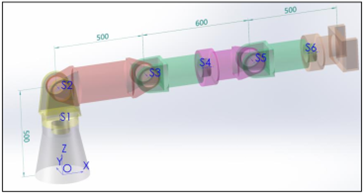
\includegraphics[width=0.5\textwidth]{Image/3.png}
	\caption{6R机器人示意图}
\end{figure}

\subsection{基于关节角操作空间的轨迹规划}
\textcolor{cherry}{\textbf{[Solution]:}首先说明,笔者这里没有采用老师在群内给出的DH参数,而是自己建立了DH参数,因为群内参考答案给出的建系参数为标准DH,而我在作业3中采用的是Modified DH,因此这里采用Modified DH建系。}参数建立同\href{https://github.com/Racheus/Robotics-Caprice/tree/master/Homework3-Kinematics}{作业三}:

\begin{table}[h]
	\centering
	\setlength{\tabcolsep}{4mm}{
	\begin{tabular}{
	>{\columncolor[HTML]{DAE8FC}}c |
	>{\columncolor[HTML]{DAE8FC}}c |
	>{\columncolor[HTML]{DAE8FC}}c |
	>{\columncolor[HTML]{DAE8FC}}c |
	>{\columncolor[HTML]{DAE8FC}}c |
	>{\columncolor[HTML]{DAE8FC}}c |
	>{\columncolor[HTML]{DAE8FC}}c }
	\hline\hline
	\diagbox{Parameter}{Joints}		 & 1           & 2           & 3             & 4            & 5            & 6            \\ \hline
	$\theta$ & $\theta_1+0$ & $\theta_2+0$ & $\theta_3-90$ & $\theta_4+0$ & $\theta_5+0$ & $\theta_6+0$ \\ \hline
	$d$      & 500         & 0           & 0             & 600          & 0            & 500          \\ \hline
	$\alpha_{i-1}$ & 0           & -90          & 0             & -90          & 90           & -90           \\ \hline
	$a_{i-1}$      & 0           & 0           & 500           & 0            & 0            & 0            \\ \hline\hline
	\end{tabular}}
	\caption{6R机器人MDH参数表}
	\end{table}

本节作业的代码参见\href{src/Rhw_5_2_1_main.m}{Click here to jump to the MATLAB code}。

基本思路是通过先通过运动学逆解,求解出三个关键节点的关节空间表达式$\boldsymbol{q}_i(i=1,2,3)$,根据这三个关键节点,通过三次样条插值,得到关节角随时间的变化,最后通过正运动学,得到末端的位置和姿态,用末端坐标系X,Y,Z三个方向的平移向量和RPY欧拉角的旋转向量随时间的变化,画出图像。

另外,笔者设置的运动时间为\textbf{$0\sim 4s$},时间间隔为$0.02s$,共计200个时间点。

\textbf{\textcolor{cherry}{关节角参数随时间的变化:}}
\begin{figure}[h]
	\centering
	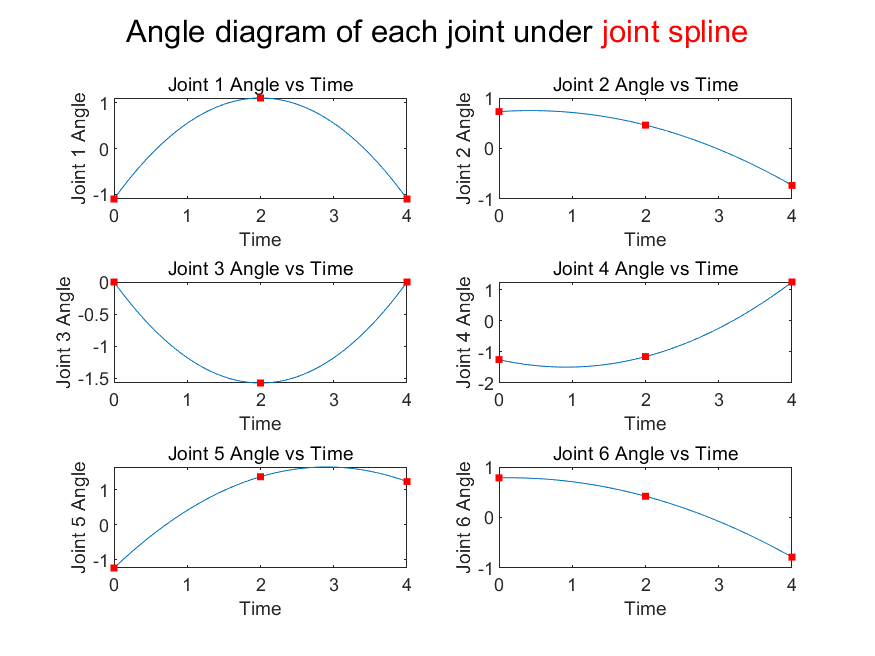
\includegraphics[width=0.65\textwidth]{Image/angle_spline_diagram.png}
\end{figure}

\textbf{\textcolor{cherry}{平移向量和旋转向量随时间变化:}}
\begin{figure}[h]
	\centering
	\subfigure[Transformation Vector]{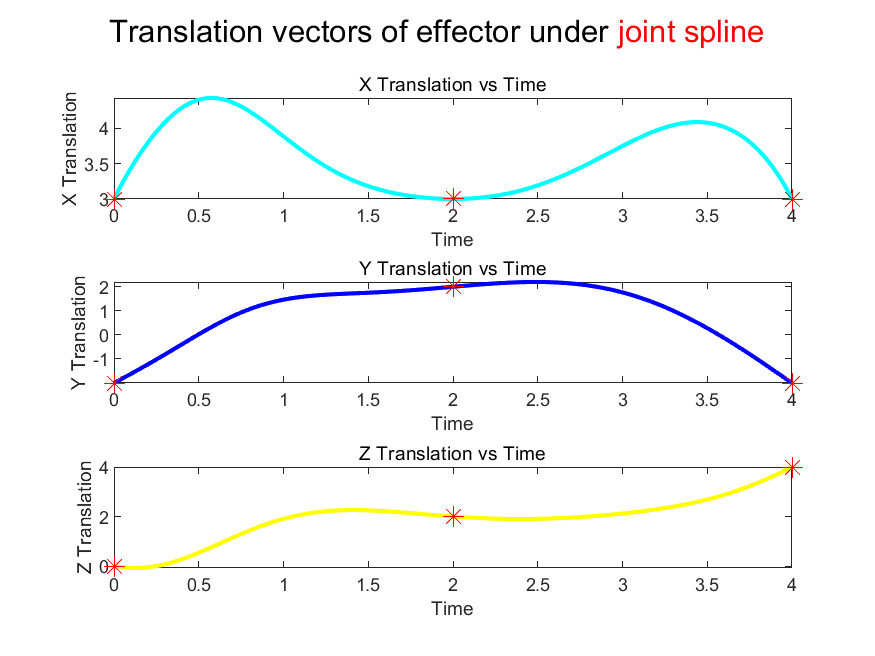
\includegraphics[width=0.45\textwidth]{Image/effector_trans_diagram.png}}
	\subfigure[Rotation Vector]{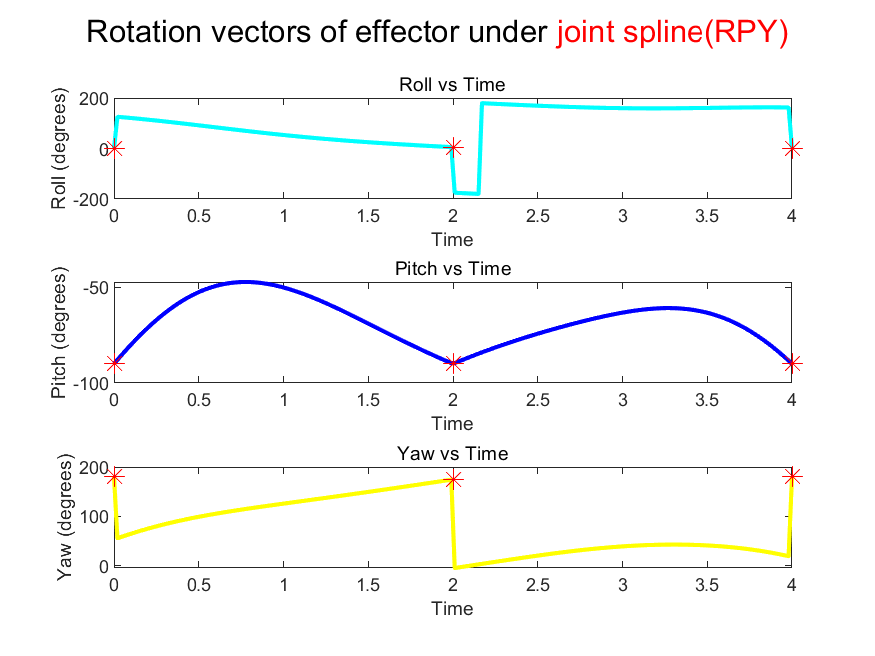
\includegraphics[width=0.45\textwidth]{Image/effector_rotation_diagram.png}}
\end{figure}

机构运动动画参见也通过上述程序一并绘出,见\href{src/robot_animation.avi}{here}。

\subsection{基于运动空间空间的轨迹规划}
\textbf{[Solution]}:本节作业的代码参见\href{src/Rhw_5_2_2_main.m}{Click here to jump to the MATLAB code}。

动画见\href{src/robot_animation_bypose.avi}{here}。

和上面类似,基本思路是找到三个目标点在空间中的坐标。将矩阵分解为旋转部分和平移部分,通过三次样条插值,得到末端的位置和姿态,用末端坐标系X,Y,Z三个方向的平移向量和RPY欧拉角的旋转向量随时间的变化,画出图像。

值得一提的是,笔者查阅相关资料,发现很多教材、教程采用的都是\textbf{四元数位姿插值},由于我们课程对这个方法没有过多要求,因此在代码编写时有所参考。还有一种方法是\textbf{球面线性插值}(Slerp): 是一种保证插值结果是有效旋转矩阵的方法。它将两个旋转矩阵之间的角度插值,然后在单位球面上进行插值。这样做可以确保插值结果是有效的旋转矩阵。我在代码文档的最后给出了\verb|slerp_rotm()|函数的一种可能实现方式。

不过观察会发现三个点处坐标系的旋转矩阵是\textcolor{cherry}{相同}的,因此本题这里的插值只需要对平移向量进行插值即可。

\textbf{\textcolor{cherry}{关节角参数随时间的变化:}}
\begin{figure}[h]
	\centering
	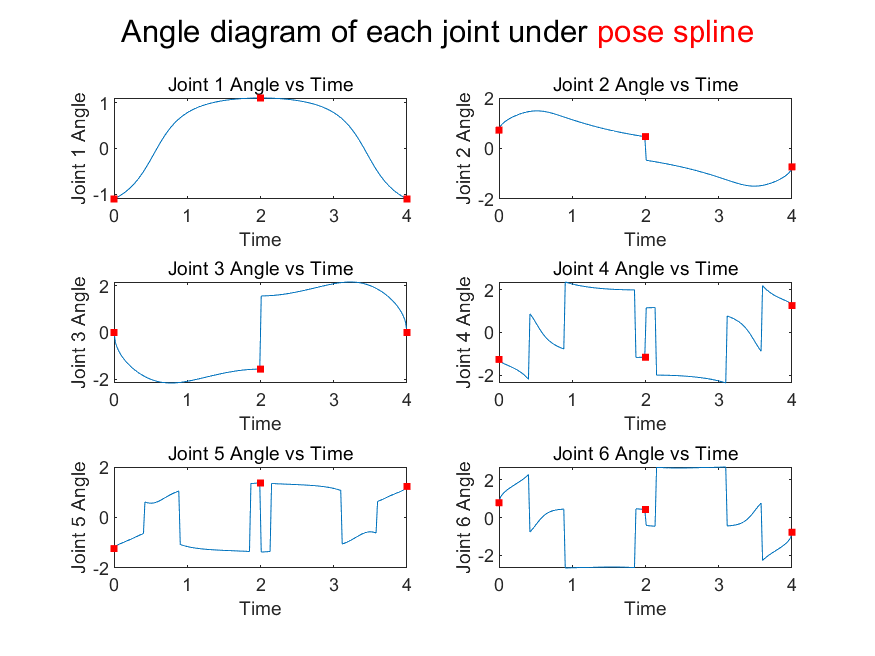
\includegraphics[width=\textwidth]{Image/angle_spline_diagram_pose.png}
\end{figure}
\newpage

\textbf{\textcolor{cherry}{平移向量随时间变化:}}
\begin{figure}[h]
	\centering
	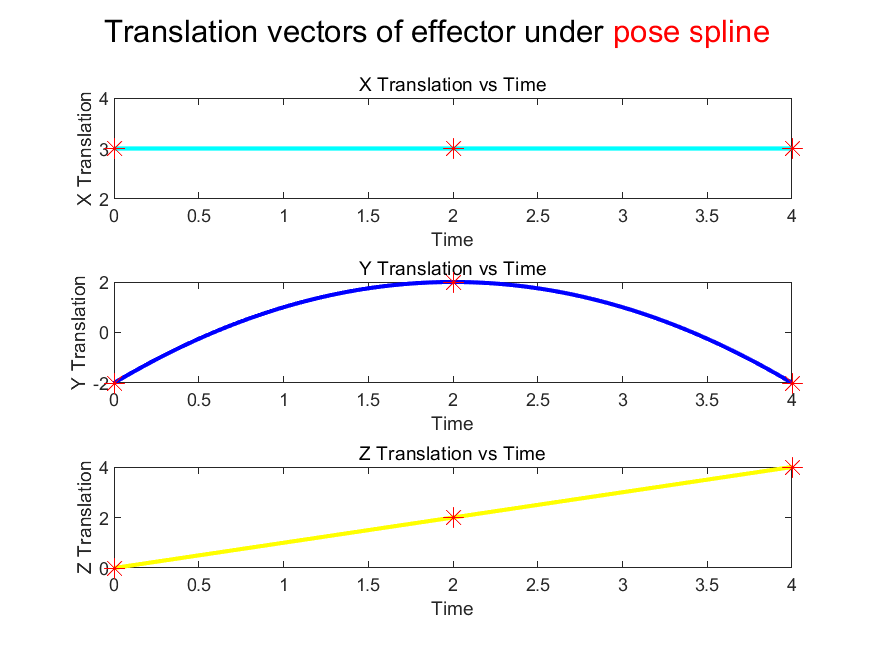
\includegraphics[width=0.6\textwidth]{Image/effector_trans_diagram_pose.png}

\end{figure}

\textbf{\textcolor{cherry}{旋转向量随时间变化:}}
\begin{figure}[h]
	\centering
	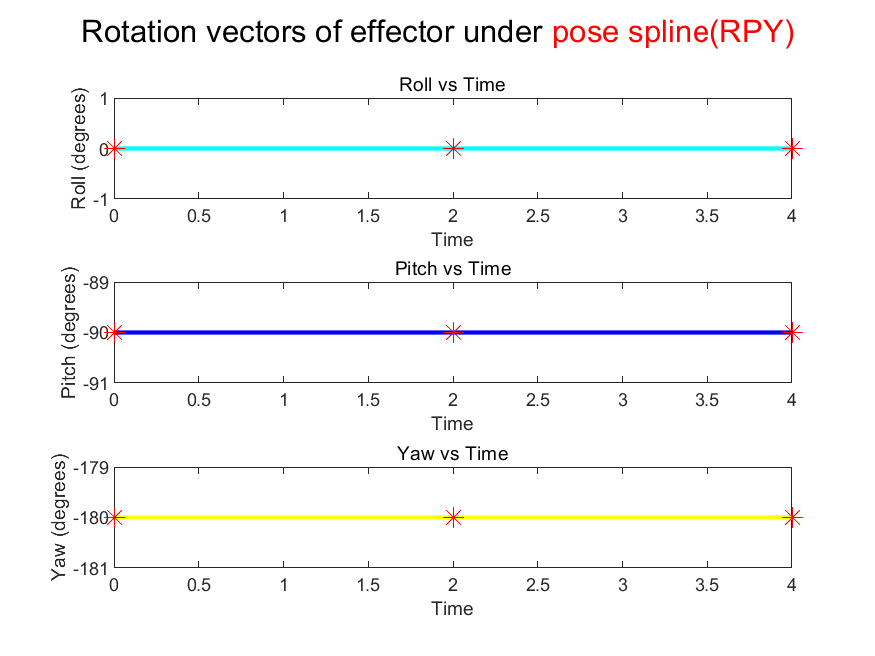
\includegraphics[width=0.6\textwidth]{Image/effector_rotation_diagram_pose.png}
\end{figure}

由上面六幅图可以看出,基于关节角操作空间的轨迹规划的轨迹更加平滑,而基于运动空间的轨迹规划的突变更大,这是因为在关节空间中,关节角的变化是连续的,而在运动空间中,末端的位置和姿态的变化是连续的,后者会导致信号的输入端突变,因此在实际应用中,需要根据具体情况选择合适的轨迹规划方法。

同样地,笔者将代码备份至\href{https://github.com/Racheus/Robotics-Caprice/tree/master/Homework5-Kinematic-Trajectory-Planning/src}{here},如果上述作业因为路径问题无法打开,麻烦助教老师查看这个链接,谢谢!
\end{document}

